
\documentclass[progress]{cmpreport}
\usepackage{hyperref}
\newcommand{\head}[1]{\textnormal{\textbf{#1}}} %Used for tables
\usepackage{fontenc}  % \textsterling for £
\usepackage{caption}

\title{Designing, Building, Coding and Tracking a Mechanical Hand/Arm}
\author{Deborah Taylor}
\registration{100085169}

\supervisor{Graeme Richards}
\date{\today}
\ccode{CMP-6013Y}

\summary{Draft as of \today.}
\acknowledgements{}

% If the figures do not fit on one page, comment this line out
\onePageLists
\linespread{1.5}
\bibliographystyle{apalike} 

% Prevents author/year errors
\usepackage{natbib}
\usepackage{float}
\usepackage{rotating}
\usepackage[strings]{underscore}
\renewcommand{\paragraph}[1]{\par\textbf{#1}\hspace{0.3em}}

\begin {document}


\section{Introduction}
Since the first industrial arm was built in 1954, by George C. Devol\footnote{George Charles Devol, Jr. American Inventor born 20 Feb 1912 and died 11 Aug 2011}, the majority have been claw based and aren't very dexterous or flexible. Due to their design restrictions they can only perform precise, repetitive tasks and are liable to fail if the claws are not aligned correctly or one stops working. \citep{devol}, \citep{grigorediscovering}.  

To increase manoeuvrability and flexibility, while also reducing restrictions, the mechanical arm needed to be redesigned so it could replicate the majority of movement in a normal hand, instead of using a claw. 

The purpose of this project is to build a bespoke mechanical (robotic) human skeletal hand/arm, code\footnote{Programming is a way of entering instructions into a machine to execute commands. Coding is another name for programming} it to pick up and put down items using relevant fingers on the hand and track items or movement. This should enable the project to develop a much more flexible hand that will allow it to work, even if one of the fingers is broken, or not in alignment. 


\section{Motivation and Aims}
Prosthetic limbs have been an interest, ever since the author's school friend developed meningitis at an early age and ended up losing an arm. The author saw how difficult it was for that person to complete even the simplest task, such as dressing or tying a shoelace. 

It would be impossible, with current skill levels and the project time-frame, to develop a fully functioning mechanical (robotic) limb, therefore, the author shifted their focus to commercial uses instead. These are much more straight forward to develop, however, if this project were to continue, the design and build could be adapted for use within health research, for prosthetic hands.

This should, hopefully, be a precursor to the author eventually moving forward into health research and development, either from a business project management perspective, or directly into Information Technology (IT) design and build.

The main aim of the project, as mentioned previously, is to design and build a mechanical (robotic) hand/arm, with coding that enables it to demonstrate the flexibility and functionality of a human hand. The hardware will be able to complete basic tasks a normal hand can process such as: moving each finger, moving the arm/hand up, down, left and right and picking up and putting down and item. It will also have more complex coding to either play "Rock, Paper, Scissors" or solve the "Towers of Hanoi puzzle". 

The author is still in the process of identifying which one of these two options will be the most suitable for this project, so the design and build has been completed so either can be coded, at a later date. Whichever option is chosen, the missing movement from the other option can be incorporated into the basic coding script, to ensure a full demonstration of flexibility is shown. 

\section{Design}
An online Trello board has been created to log each task, within the project. This enables the author to continually monitor progress and ensure all tasks are completed correctly. To view this Trello board access: https://trello.com/b/cdHgyGX0.

This project involves both hardware and software so a Software Engineering Design Document is needed to show designs, development and testing \footnote{A Design Document is a technical guide for Developers and includes Definitions, Requirements, Use Cases, etc.}. This has been identified as the best way to make sure each stage of the design and build is completed correctly and efficiently \citep{mcelrath}.

The Document created is too large to include in this report so an overview has been covered here. It starts with an \textit{Introduction, Glossary}\footnote{Glossary: helps clarify definitions so the reader can understand the vocabulary used}, \textit{Similar Systems Analysis}\footnote{Similar Systems Analysis: a way of identifying if there were any "on the shelf" hardware that can be used and, if not, identify if anything currently in use can be adapted for this project} and then moves onto a \textit{MoSCoW} analysis:

\subsection{MoSCoW}
This process determines the different requirements that will be in and out of scope for the project, along with how they should be prioritised for development. This analysis is made up of \textit{Must Have, Should Have, Could Have, Won't Have} tasks. See below: \newline

\textbf{\underline{\large{Must Have:}}}

The \textbf{\textit{Must Have}} tasks are identified as absolutely necessary, at base level, for the project to work. These will be prioritised within development and the next section will not be started until these are fully completed and tested. 

\begin{itemize}
	\item \textit{Skeletal hand design and arm (up to the equivalent of an elbow)}
	\item \textit{Fingers and thumb that can move independently or together}
	\item \textit{Movement rotation of 90 degrees, up, down, left and right}
	\item \textit{Coding to enable movement of the arm: up, down, left and right}
	\item \textit{Coding to enable the hand to pick up, hold and put down an item} %\newline \newline
\end{itemize} 

\textbf{\underline{\large{Should Have:}}}

The \textbf{\textit{Should Have}} tasks are identified as necessary to the project to increase effectiveness within the design. These are the second stage of a development and will only be started, completed and tested, once the \textit{Must Have} tasks are working correctly.

\begin{itemize}	
	\item \textit{Coding to enable the hardware to play Rock, Paper, Scissors or solve Towers of Hanoi puzzle}
	\item \textit{Sensor or Camera connected to the hardware (with or without a wire) to identify items or movement}
\end{itemize}	

\textbf{\underline{\large{Could Have:}}}

The \textbf{\textit{Could Have}} tasks are identified as not absolutely critical to the project.  These are tasks which are desired and could be implemented, depending on cost and the time-frame available. 
\begin{itemize}	
	\item \textit{Ability to move independently of a PC or laptop (utilising a servo controller mounted on the arm)}
	\item \textit{Haptic sensors to enable feedback on how the hand grips an item}
\end{itemize}

\textbf{\underline{\large{Won't Have:}}}

The \textbf{\textit{Won't Have}} tasks are identified to be out of scope for the project and will not be implemented. If the project were to continue into a future development stage, these could be implemented then.  

\begin{itemize}		
	\item \textit{Independent thought and movement eg Artificial Intelligence }
\end{itemize}

Once the \textit{MoSCoW} analysis has been completed a Use Case (UML) diagram\footnote{Unified Modelling language (UML) is a standard modelling language for developers to visualize and document tasks} is designed, using the above priorities, to show User interaction with the hardware \citep{AljamaanLBGF14}. See figure 1 below:

\begin{figure}[H] 
	\caption{UML Use Case Diagram }
	\centering
	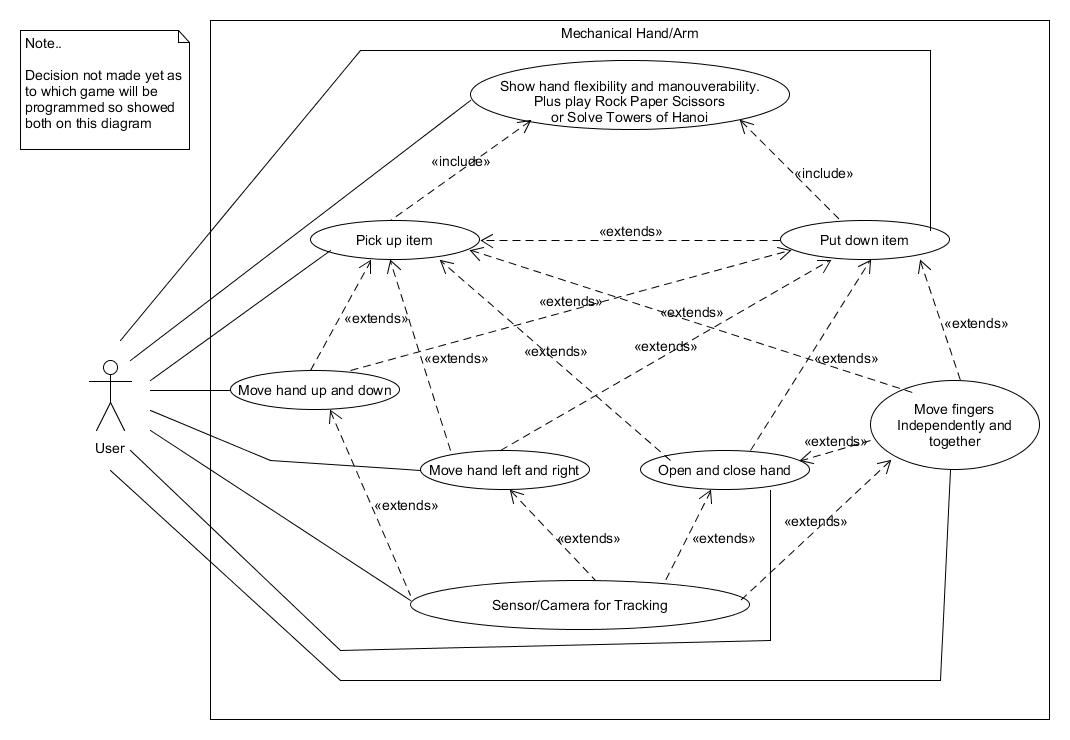
\includegraphics[width=1 \textwidth, height=0.6 \textheight]{photos/UMLdiagram.jpg}
\end{figure}

Following completion of this \textit{Use Case UML diagram}, \textit{Use Case descriptions}\footnote{Use Case Descriptions are written descriptions of how users will perform tasks.} are created for each of the tasks shown in the diagram. See below for an example of a \textit{Use Case Description} for opening the hand:

\begin{itemize}		
	\item \textit{Use Case 3 Open Hand: describes the process of connecting the laptop signal to the Hand hardware and enabling the Hand to open. This is a basic command that will be fundamental to the Hand movement for later, more complex coding.}
\end{itemize}

This then leads onto each description being expanded and \textit{Detailed Use Cases} being created. These \textit{Detailed Use Cases} show the steps required to achieve each task eg triggers, frequency and release schedules, along with providing information needed for development. See figure 2 below for an example of the \textit{Open Hand Use Case} created for this project:
\begin{figure}[H] 
	\caption{Use Case Open Hand Example }
	\centering
	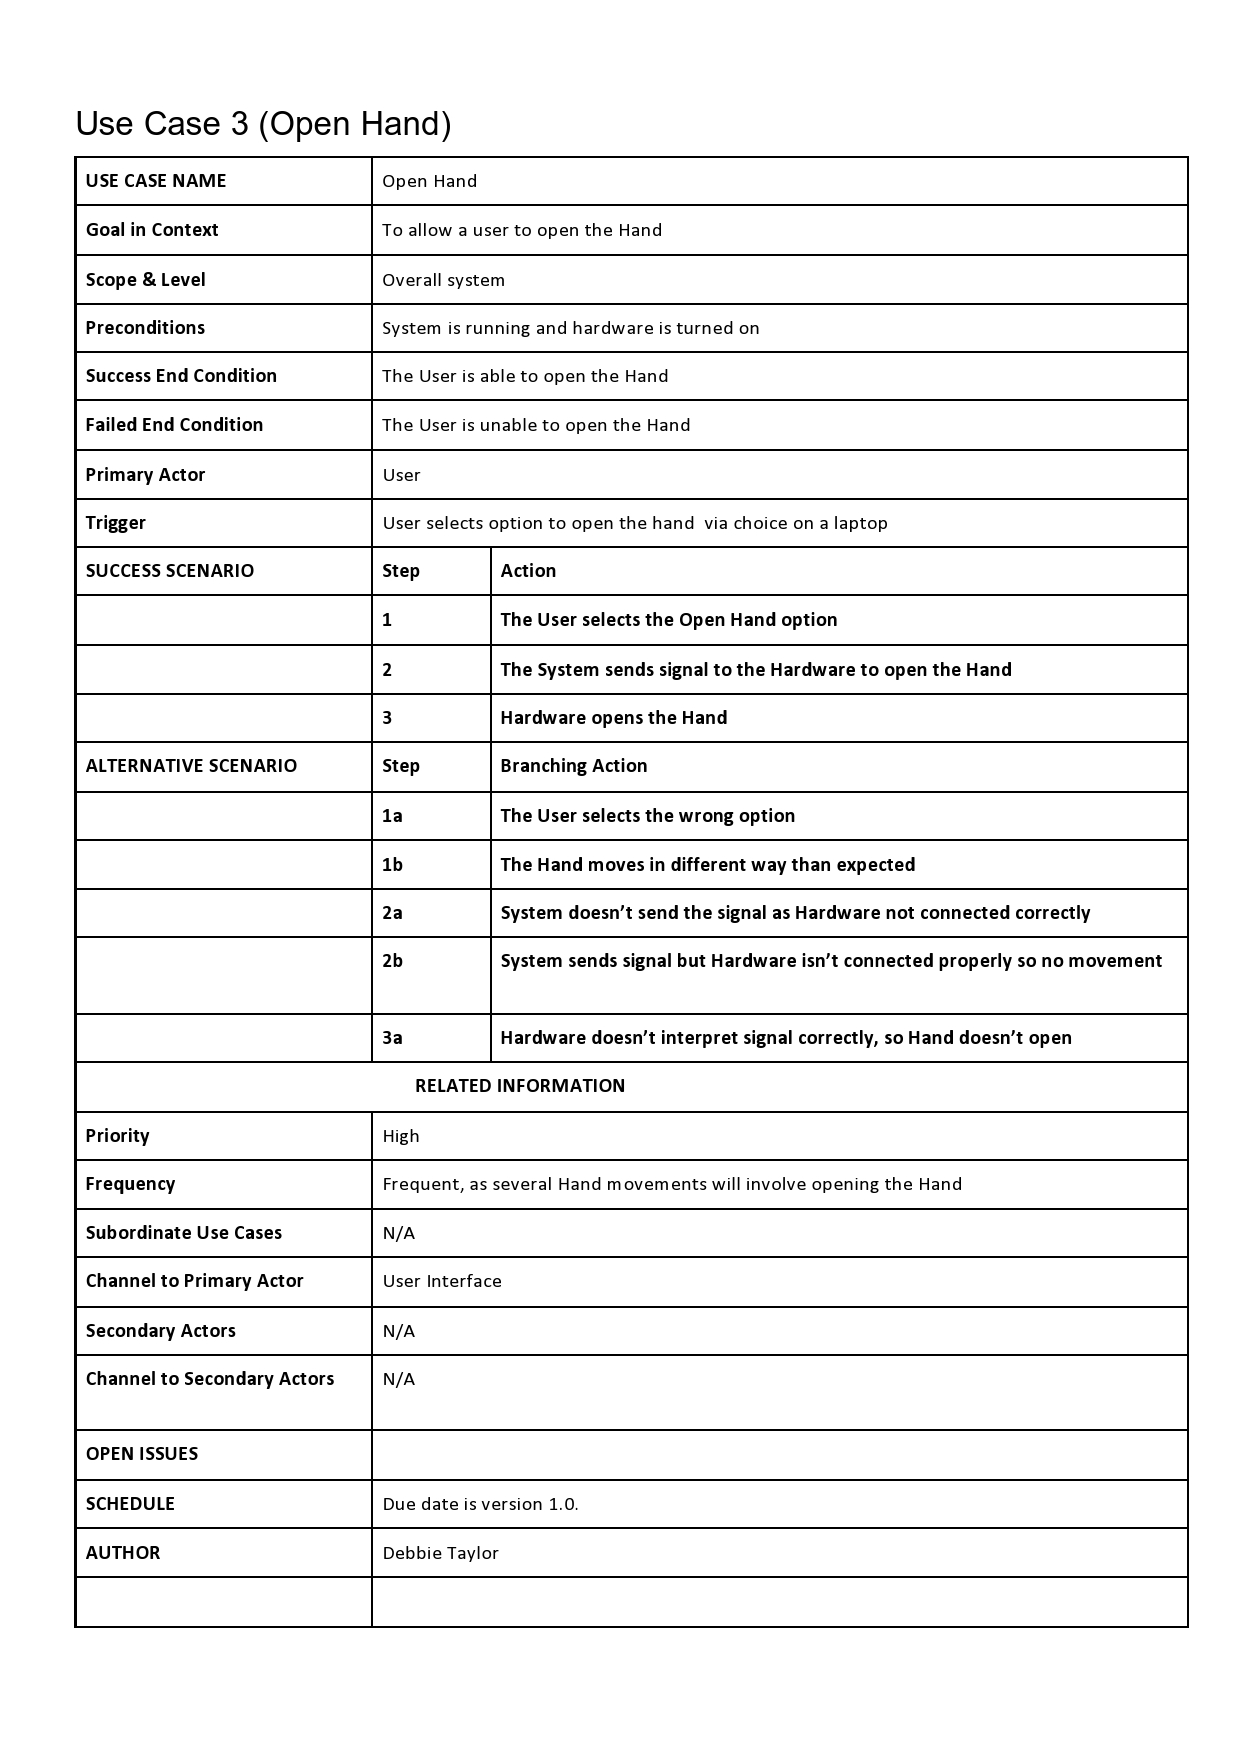
\includegraphics[width=1 \textwidth, height=0.76 \textheight]{photos/Use Case_OpenHand.jpg}
\end{figure}

Once the \textit{Detailed Use Cases} are completed the final stage\footnote{As this is a hardware and software design there is no need for Architecture diagrams etc} of this Design Document is to create \textit{Sequence Diagrams}. These show step by step representations of a specific scenario. See figure 3 below, showing an example of the steps needed for the hardware to open the hand: 

\begin{figure}[H] 
	\caption{Sequence Diagram Example }
	\centering
	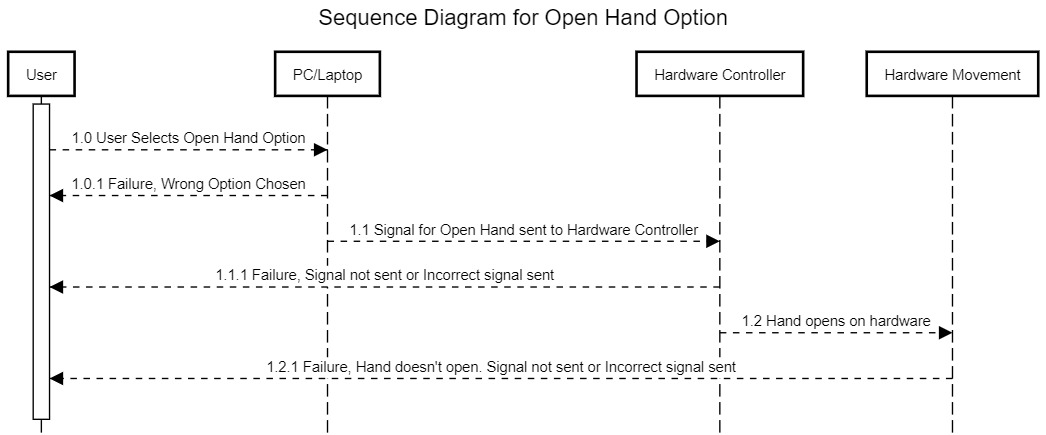
\includegraphics[width=1 \textwidth, height=0.3 \textheight]{photos/sequence_diagram.jpg}
\end{figure}

Completing this Design Document confirmed there is no "off the shelf" skeletal hand/arm hardware available, so a bespoke build was required for this project.

\section{Hardware Build}
The first stage of the build was to identify how a human hand works. In order for the hand to open, close, move each finger, hold items etc, a combination of the fingers and thumb need to be working in sequence \citep{freivalds2011biomechanics}. 

Identifying this information enabled the author to specify exactly which metal shapes needed to be cut and how many servos, joints etc were needed to build the hardware. A friend of the author is a machinist and he agreed to cut the bespoke parts, with the rest of the equipment parts being obtained "off the shelf", such as Arduino servos, wiring, sensors and a Polulo servo controller unit for mounting on the arm. See figure 4\footnote {Source: http://visual.merriam-webster.com/human-being/anatomy/skeleton/hand.php} below for the picture the author used to identify the shapes needed to build a skeletal human hand:

\begin{figure}[H] 
	\centering
	\caption{Bones and Joints of the Human Hand.} 
	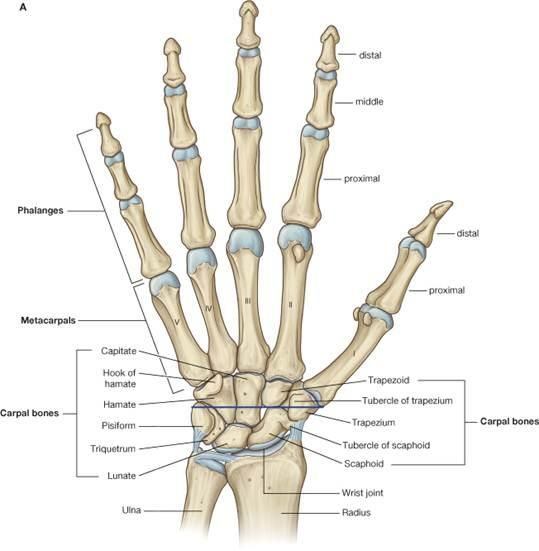
\includegraphics[height=0.4\textheight, keepaspectratio]{photos/hand.jpg} 
\end{figure}

Due to the hardware being fundamental to the project, the build started during the summer holidays and continued until the middle of Semester 1. Multiple photographs were taken showing step by step progress. See figure 5 and figure 6 below for a selection of four photographs showing the build as it progressed: 

\begin{figure}[H]
	\centering
	\caption{Hardware Build Progress - Zero to hand completion }
	\begin{tabular}{ll}
		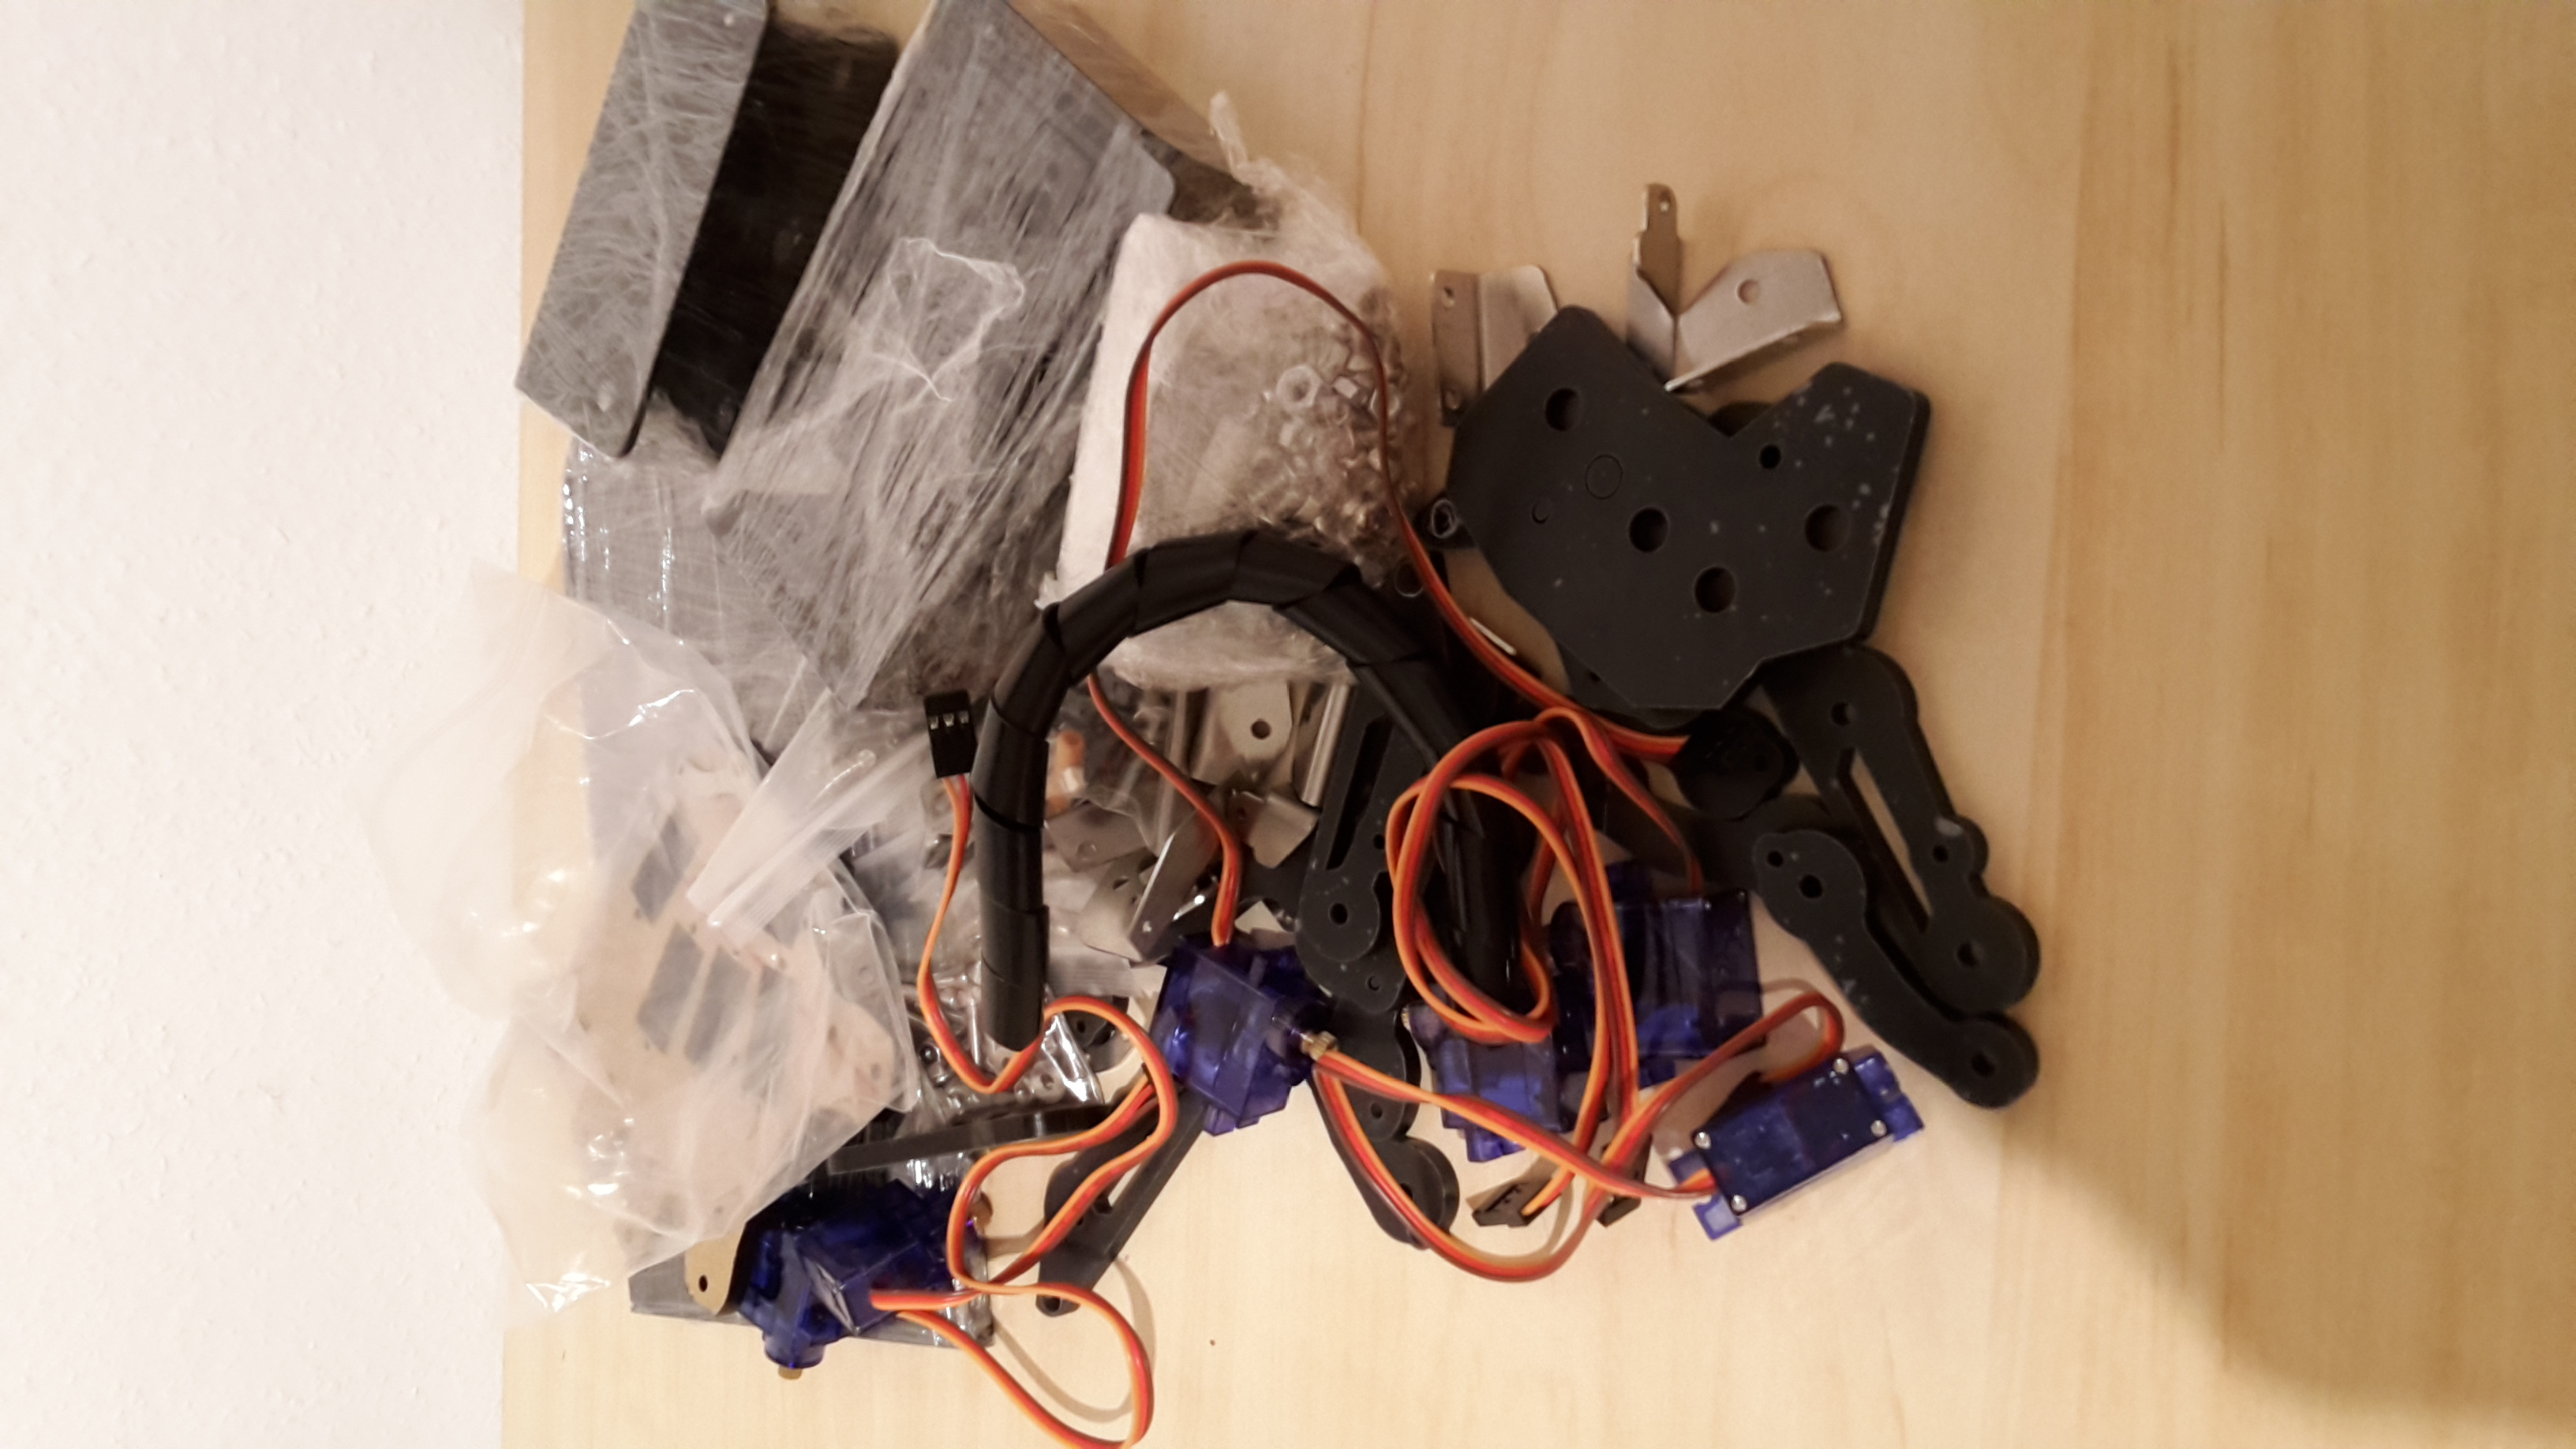
\includegraphics[trim=2cm 2cm 3cm 4cm, clip=true, totalheight=0.15\textheight, angle=0]{photos/Day 1.jpg}
		&
		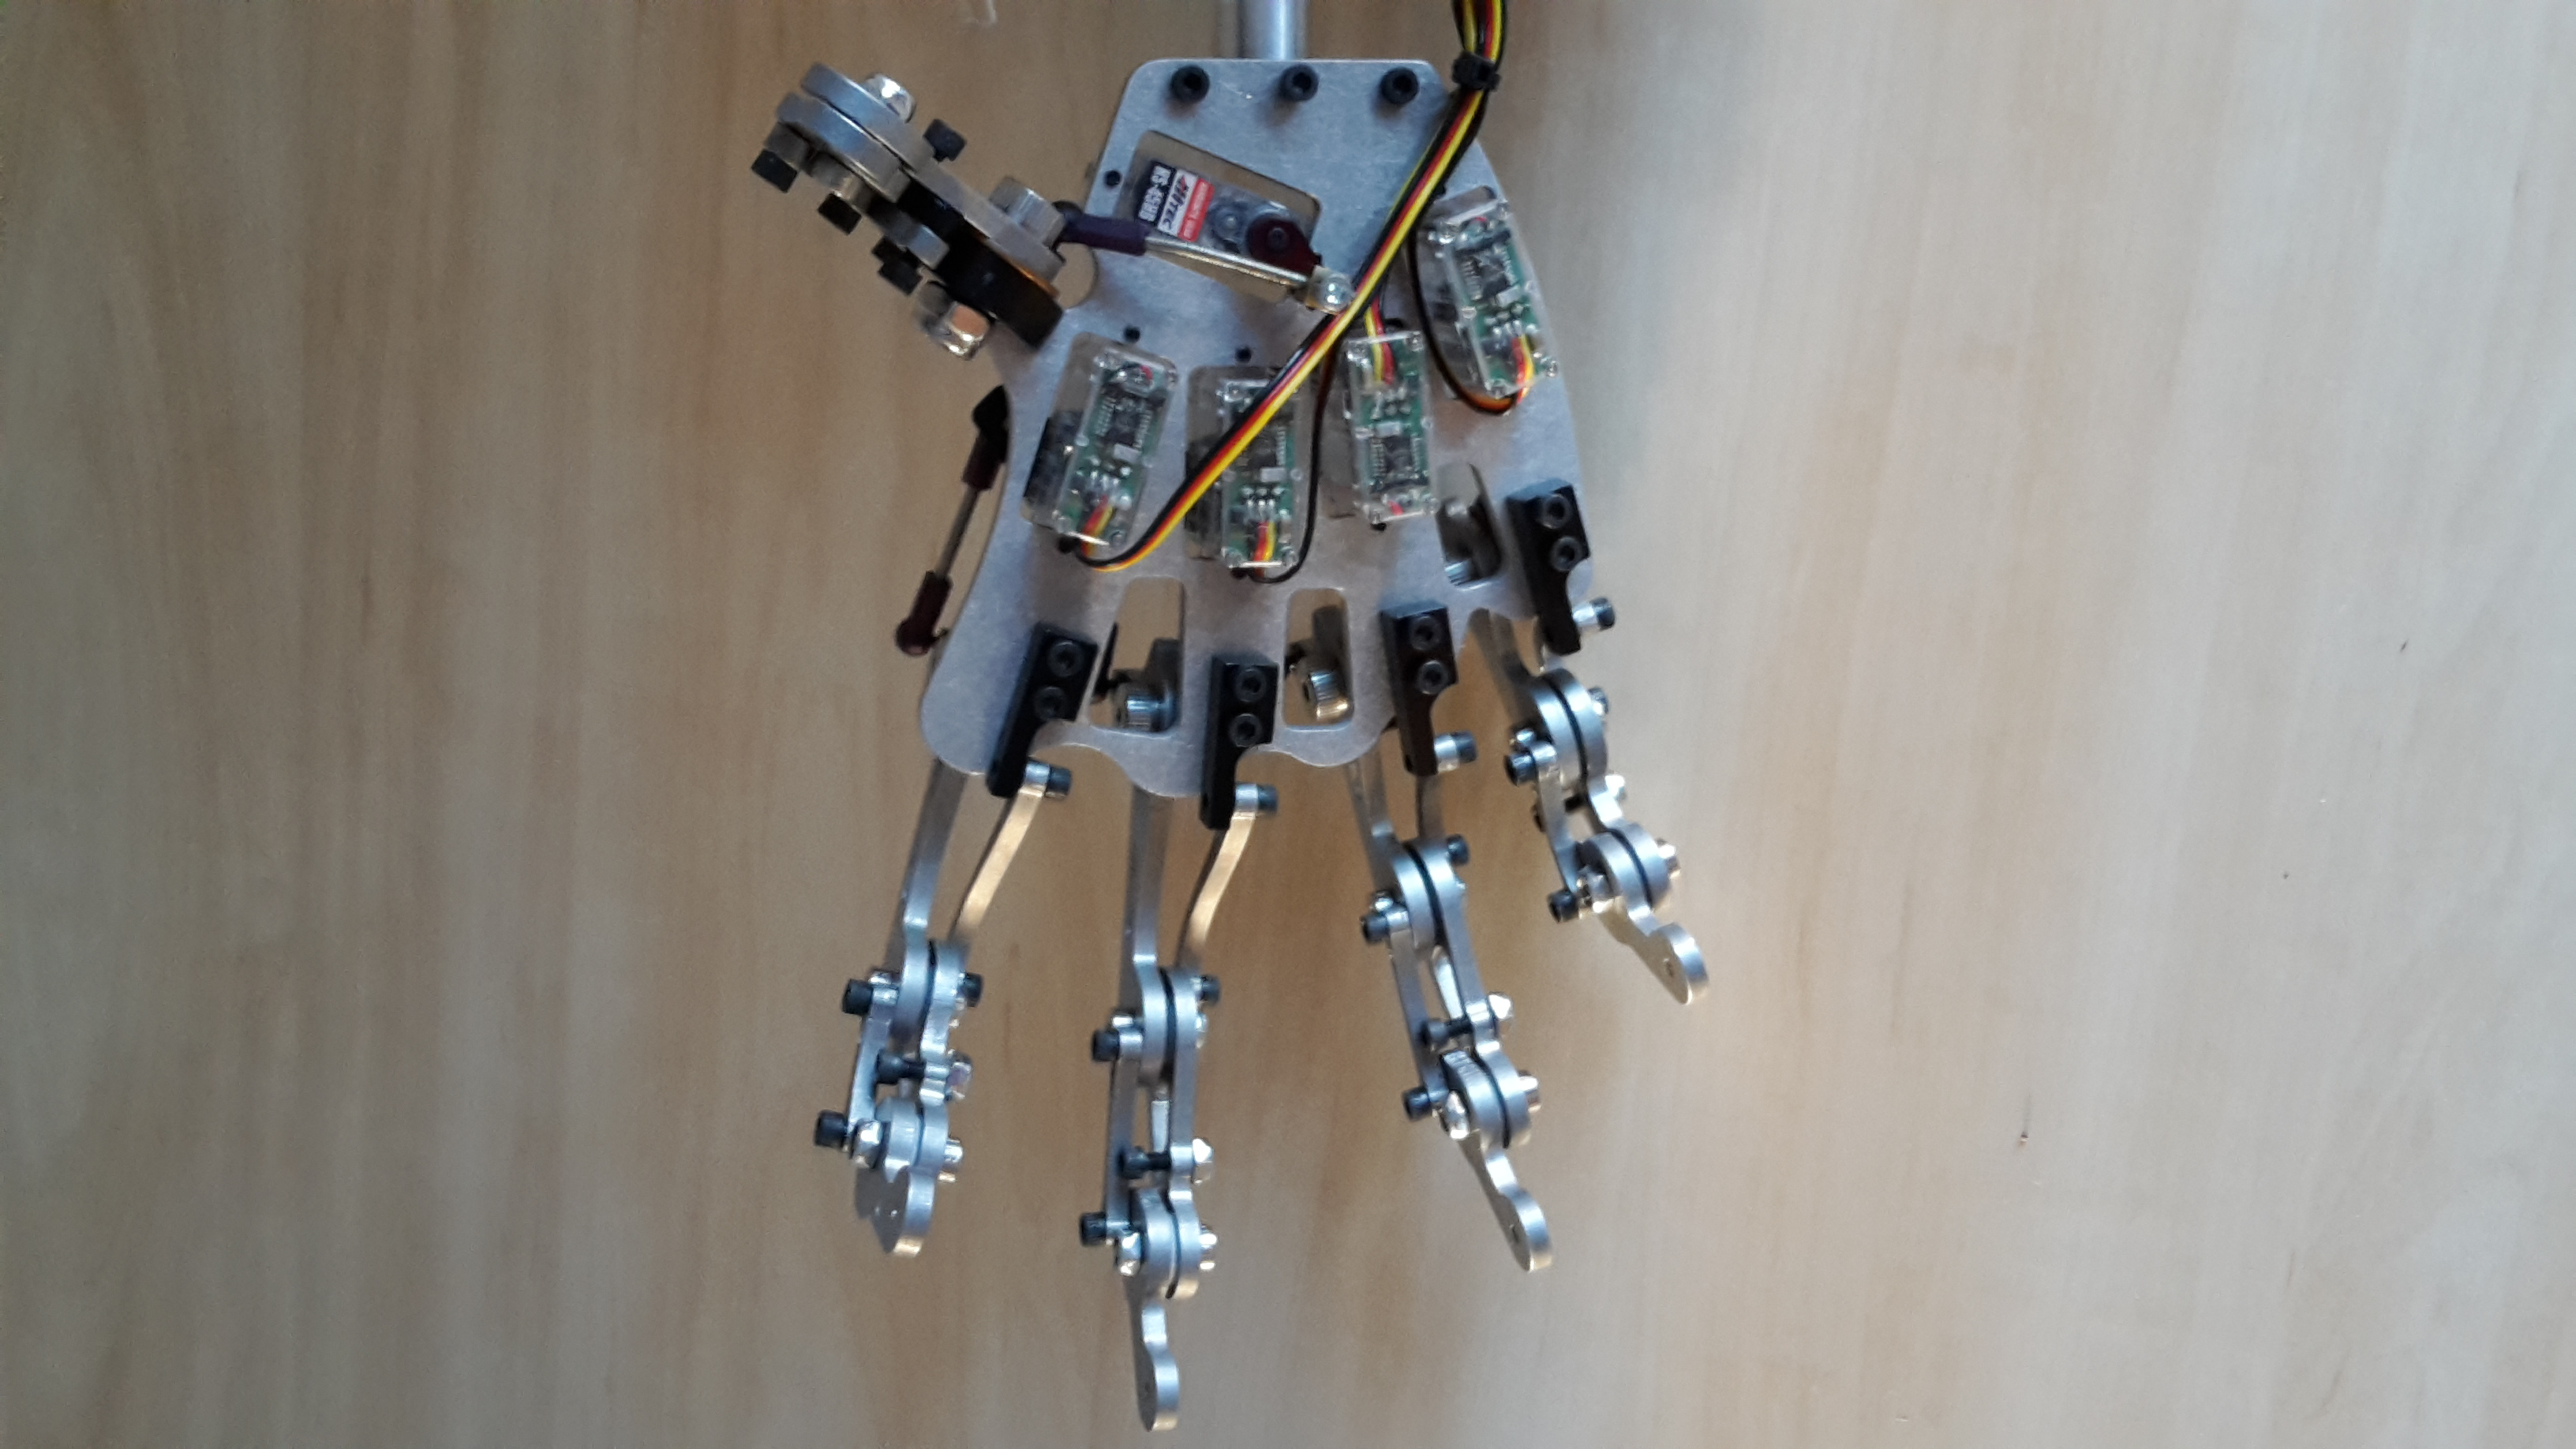
\includegraphics[trim=2cm 2cm 3cm 4cm, clip=true, totalheight=0.15\textheight, angle=0]{photos/Day 10.jpg}
	\end{tabular}
\end{figure}

\begin{figure}[H]
	\centering
	\caption{Hardware Build Progress - Arm and base to Full build completion }
	\begin{tabular}{ll}
		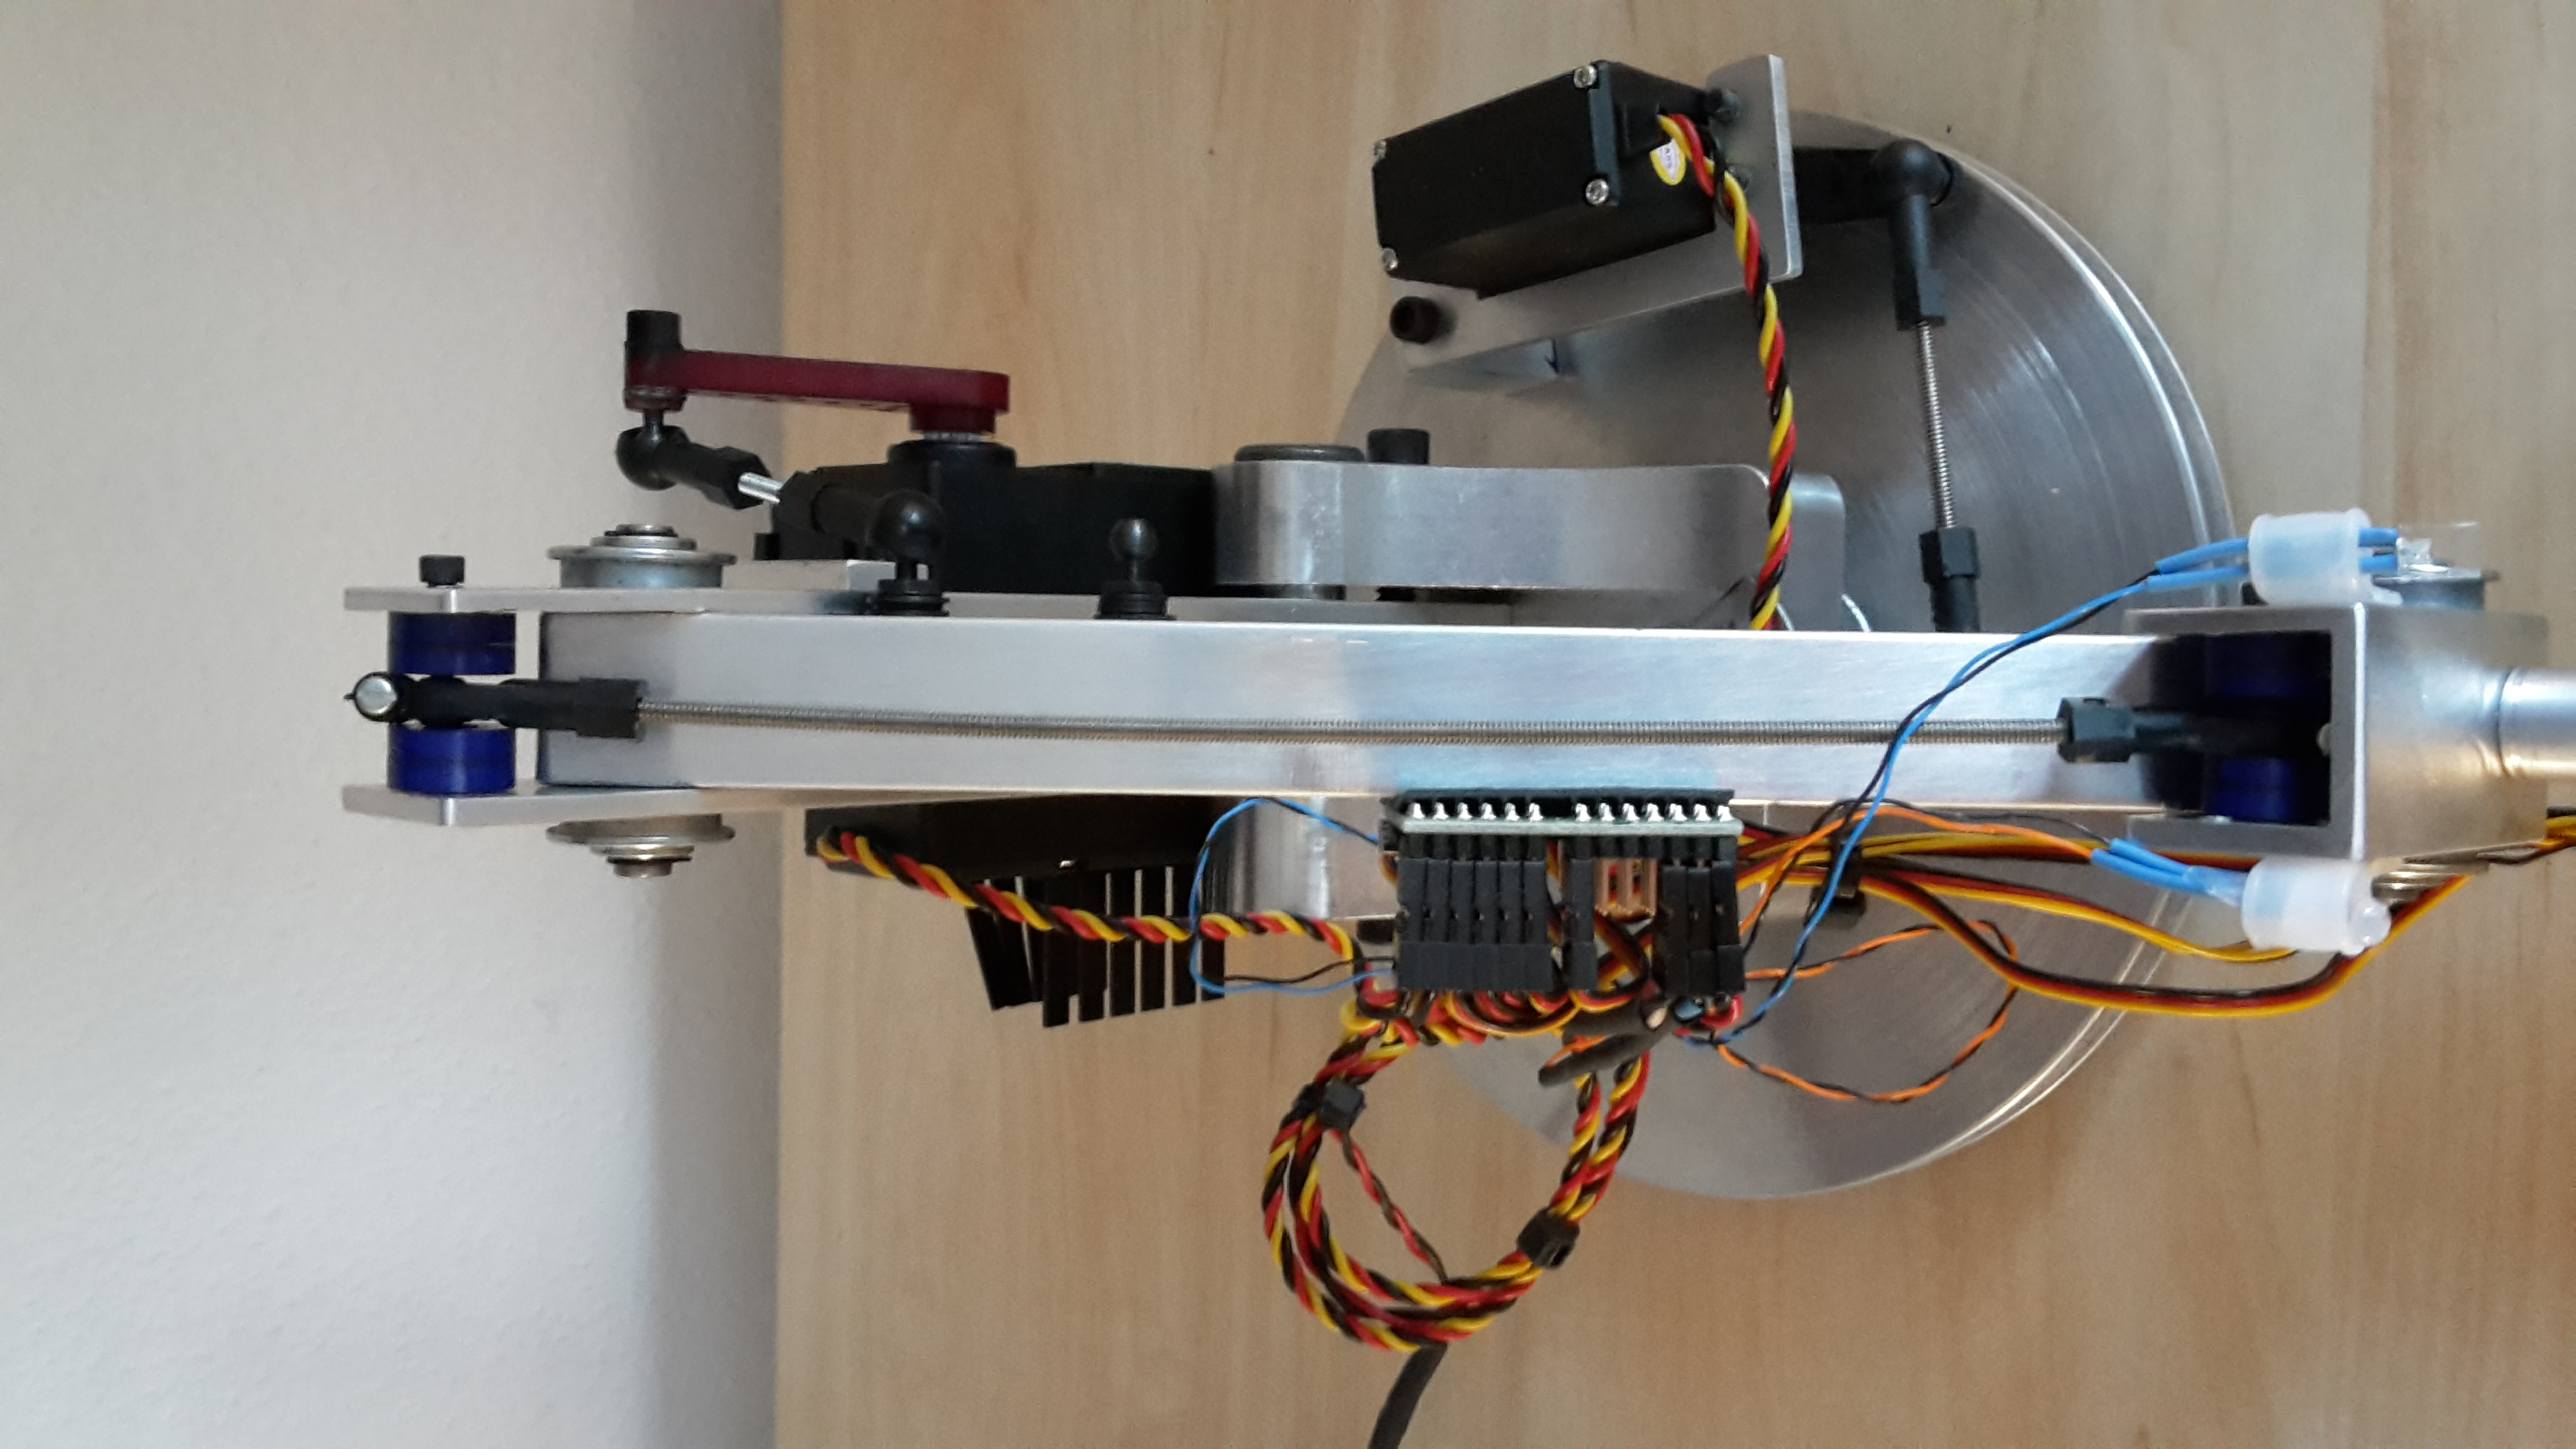
\includegraphics[trim=2cm 2cm 3cm 4cm, clip=true, totalheight=0.15\textheight, angle=-90]{photos/Day 36-pt1.jpg}
		&
		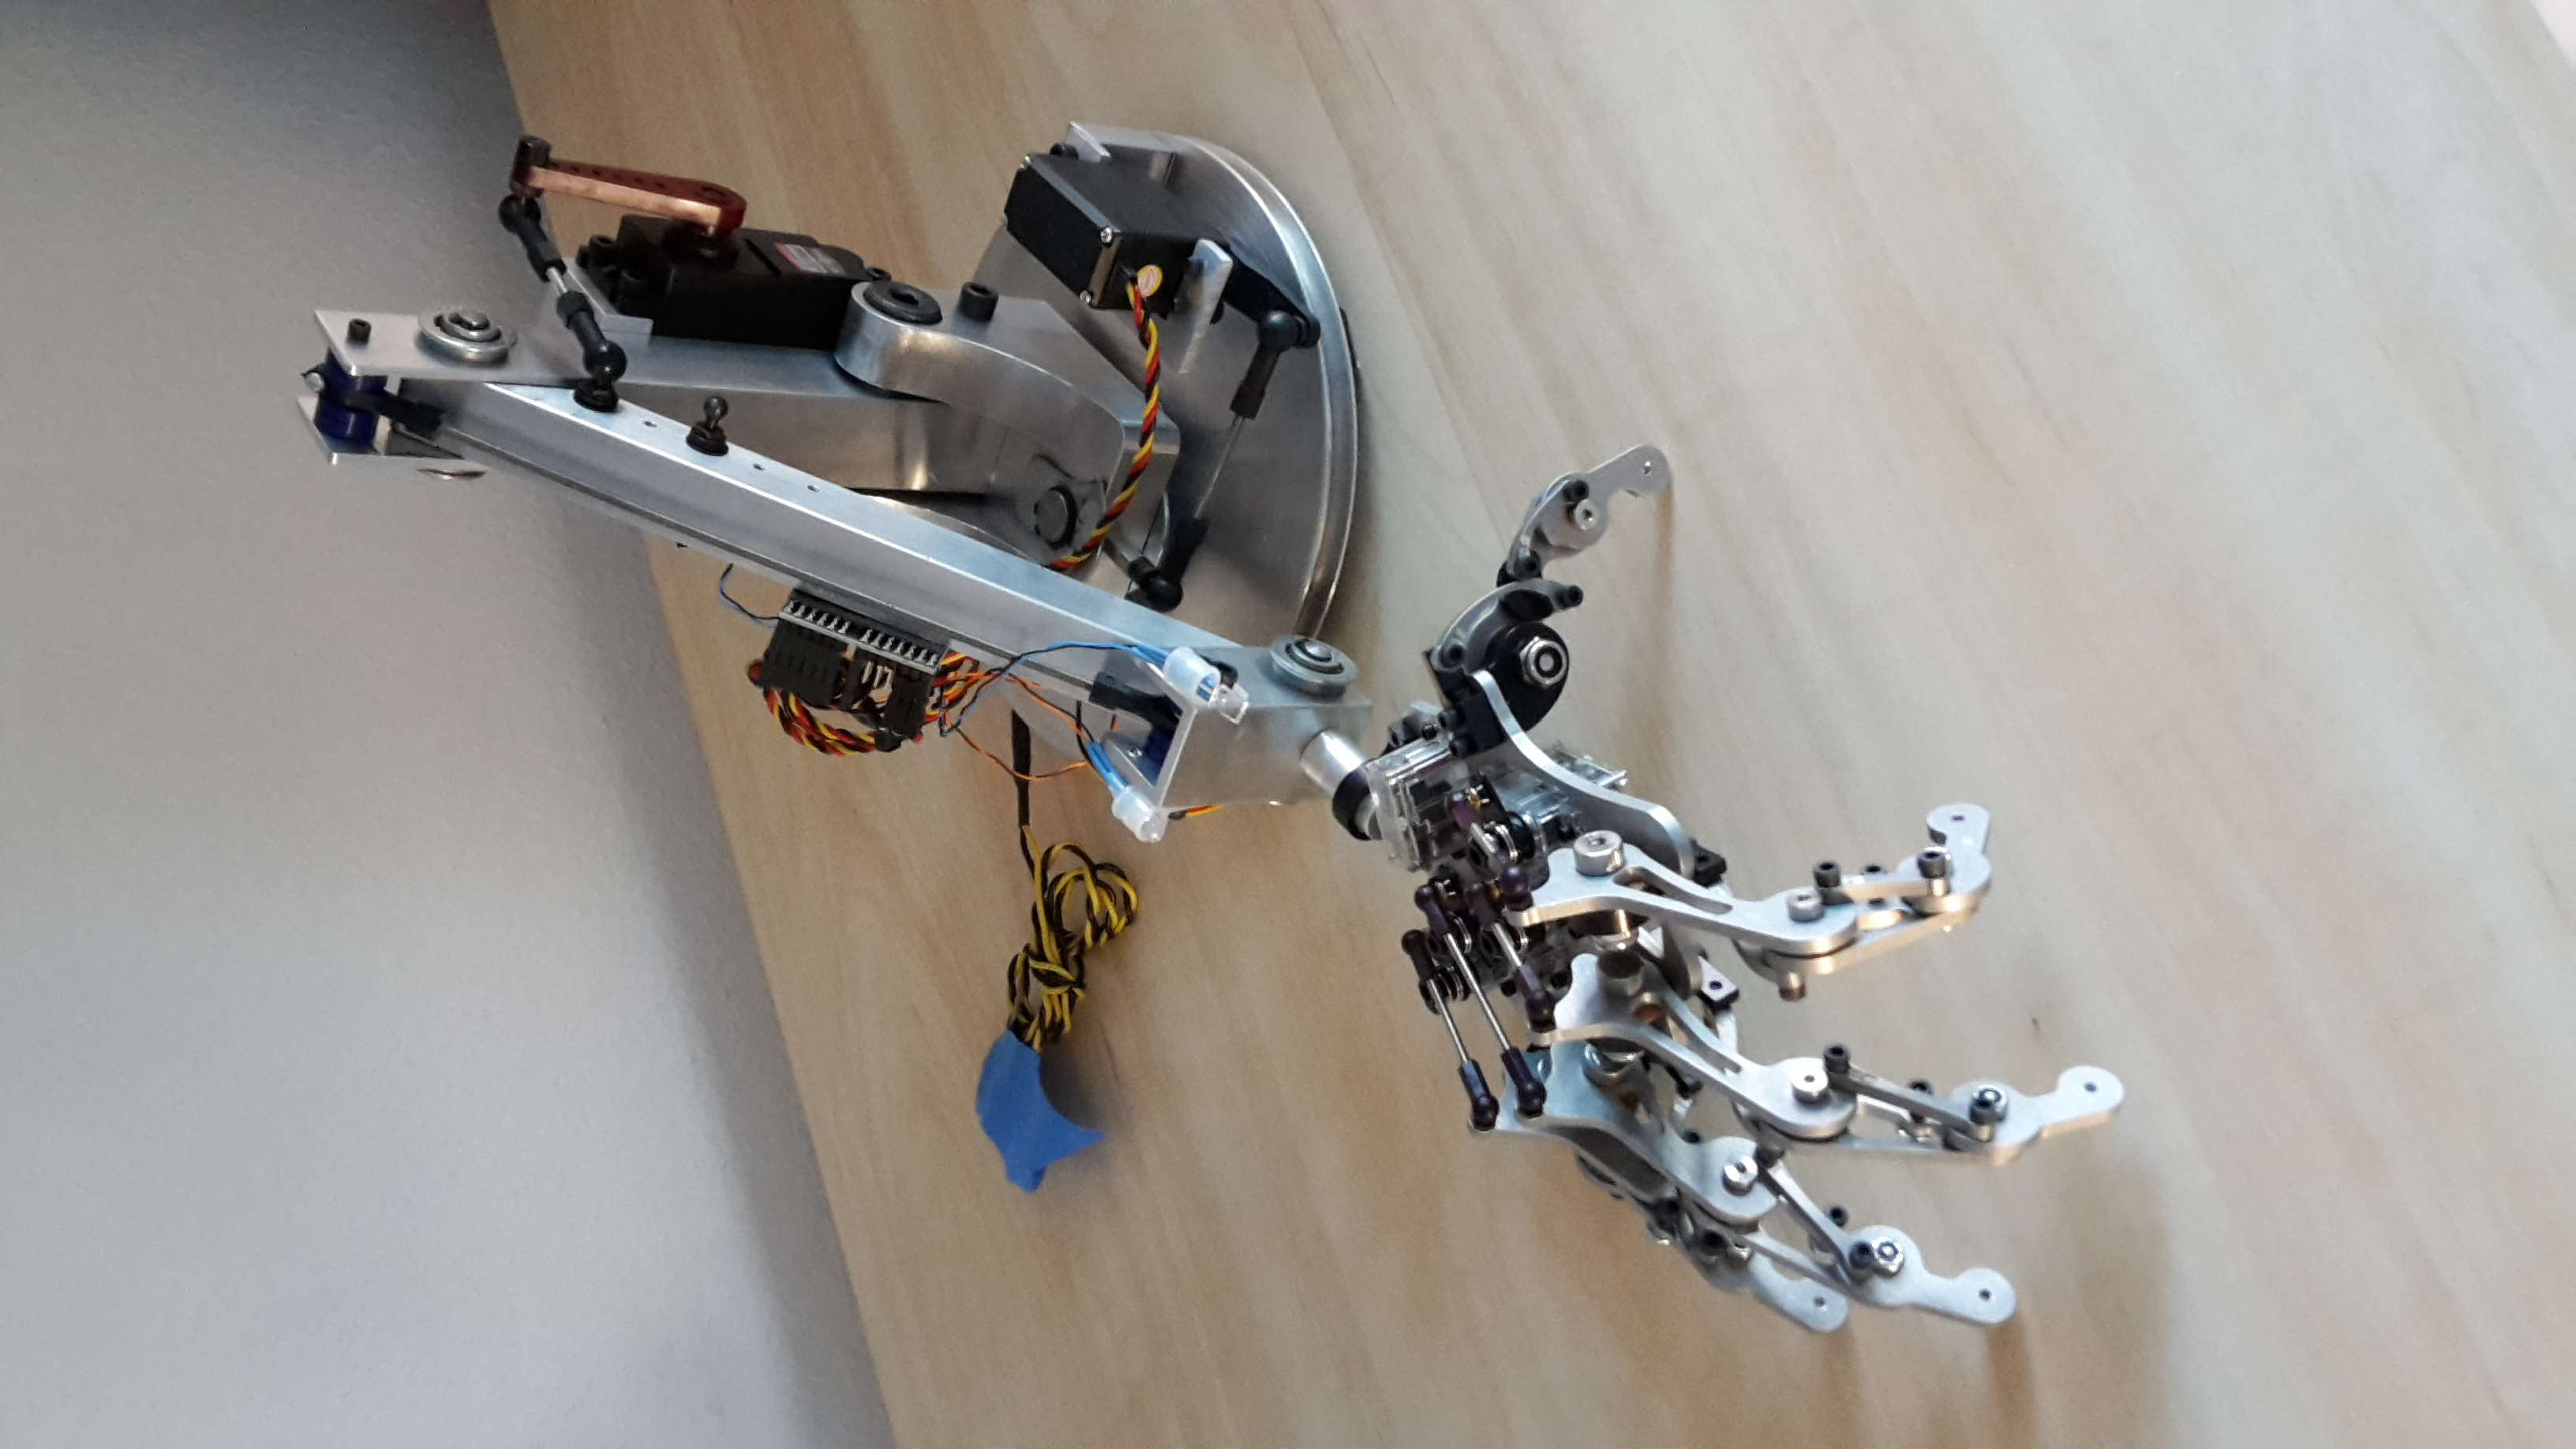
\includegraphics[trim=2cm 2cm 3cm 4cm, clip=true, totalheight=0.15\textheight, angle=-90]{photos/Day 42-pt5.jpg}
	\end{tabular}
\end{figure}

The build didn't quite go to plan, as the author estimated it would take about three full weeks, however it ended up taking just over seven. The hand and arm itself was much more fiddly to put together than expected and there were several welding issues before the parts were fully positioned correctly. Also, when first tested the original servos were not strong enough to move the hand, so stronger ones had to be ordered. Once replaced and tested again, the second ones were found to be too strong and blew some fuses and the plug. It was, therefore, back to the drawing board to identify the correct sizes needed, but finally the correct servos were obtained and the build was completed.

\section{Progress and Contingencies}
With the build completed half way through Semester 1, the hardware was ready for the basic coding. This coding script is now written and the hand can currently move up, down, left, right, hold a coffee cup, move it and put it down. 

This means the \textbf{\textit{Must Have}} section of the \textit{MoSCoW} is fully completed and tested, leaving the more complex tracking coding  (\textbf{\textit{Should Have}} section) now ready to be started.

At the end of this report are two project Gantt Charts. The first (figure 7) shows the original version included in the Project Proposal. Unfortunately, due to a personal family bereavement the project needed to be placed on hold for a few weeks. The plan, therefore, needed to be changed in order to keep the project on target. 

The original plan showed the Christmas holidays as unused so, from a contingency viewpoint, this is now being included in the revised plan. The remaining tasks have also been revised, with new time-lines, to ensure the project remains on target for the original completion date. See the second Gantt chart (figure 8) for the revised plan.

\section{Evaluation}
Following careful reflection and evaluation the author feels that, even with the unexpected delay on the more complex coding, good progress is being achieved with this project. 

The hardware build and basic coding took a lot longer than expected, and was a lot more complicated than originally considered, when the project was proposed. Some of the parts also took longer than expected to arrive and, as described above, some had to be re-ordered and re-inserted into the hardware due mistakes by the author. This was expected, as the author had never processed anything like this before, so was covered by the project being started during the summer holidays, instead of being left until the Semester started in September.

If this had not been started early the unexpected delay, mentioned above in the Progress and Contingencies section, would have fallen during the \textit{Must Have} stage of development, rather than the \textit{Should Have} stage, which would have made it a lot more difficult to regain control. 

Overall the skill level of the author, for electronics and understanding how software code interacts with hardware, has increased considerably since the start of the project. Any mistakes made, were learnt from and would not be made again, in future projects.

Progress will continue to be closely monitored during the second half of the project, to ensure no further delays occur and any potential issues are dealt with quickly and efficiently. This will be achieved by the author using Trello to keep tasks on target, having regular meetings with their project supervisor and with careful project management of their available time during Semester 2.

   \begin{cmpfigure}{Original Project Gantt chart time-table\label{pplan}}
 	\centering
 	\begin{sideways}
 		\newganttchartelement{voidbar}{voidbar/.style={draw=black, top color=black!25, bottom color=black!23}}
 		
 		\begin{ganttchart}[x unit=0.45cm, vgrid, title label font=\scriptsize,canvas/.style={draw=black, dotted}]{1}{34}
 			\gantttitle{Project schedule shown for e-vision week numbers and semester week numbers}{34} \\
 			\gantttitlelist{8,...,41}{1}\\
 			\gantttitlelist{1,...,12}{1}
 			\gantttitle{Christmas}{4}
 			\gantttitlelist{1,...,9}{1}
 			\gantttitle{Easter}{4}
 			\gantttitlelist{10,...,14}{1}\\
 			
 			% Numbered in order of declaration, zero based
 			
 			\ganttbar{Project proposal}{1}{3} \\ %elem0
 			\ganttbar{Literature review}{2}{5} \\ %elem1
 			\ganttbar{Complete design and build}{2}{4} \\ %element 2
 			\ganttbar{Basic coding and testing}{4}{8}\\ %element3
 			\ganttmilestone{Basic code delivery}{9} \\ 
 			\ganttbar{Investigate Tracking}{9}{10}\\ %element 5
 			
 			\ganttbar{Tracking coding}{10}{12} %element 6 & don't include \\ to keep on same line
 			\ganttvoidbar{}{13}{16}  %don't include \\ to keep on same line
 			\ganttbar{}{17}{21}\\
 			
 			\ganttbar{Test Tracking code}{17}{22}\\
 			
 			\ganttbar{Review and Evaluation}{21}{25} \\
 			\ganttmilestone{Completed code delivery}{25} \\  
 			\ganttbar{Final report writing}{23}{30} \\  %work on writing over Easter
 			\ganttbar{Inspection preparation}{31}{34}
 			
 			\ganttlink{elem0}{elem2}
 			\ganttlink{elem1}{elem2}
 			\ganttlink{elem2}{elem3}
 			\ganttlink{elem3}{elem4}
 			\ganttlink{elem4}{elem5}
 			\ganttlink{elem5}{elem6}
 			%elem 6-7 not needed as void   
 			\ganttlink{elem8}{elem9}
 			\ganttlink{elem9}{elem10}
 			\ganttlink{elem10}{elem12}
 			\ganttlink{elem11}{elem13}
 			
 		\end{ganttchart}
 	\end{sideways}
 \end{cmpfigure}

 \begin{cmpfigure}{Revised Project Gantt chart time-table\label{pplan}}
 	\centering
 	\begin{sideways}
 		\newganttchartelement{voidbar}{voidbar/.style={draw=black, top color=black!25, bottom color=black!23}}
 		
 		\begin{ganttchart}[x unit=0.45cm, vgrid, title label font=\scriptsize,canvas/.style={draw=black, dotted}]{1}{34}
 			\gantttitle{Project schedule shown for e-vision week numbers and semester week numbers}{34} \\
 			\gantttitlelist{8,...,41}{1}\\
 			\gantttitlelist{1,...,12}{1}
 			\gantttitle{Christmas}{4}
 			\gantttitlelist{1,...,9}{1}
 			\gantttitle{Easter}{4}
 			\gantttitlelist{10,...,14}{1}\\
 			
 			% Numbered in order of declaration, zero based
 			
 			\ganttbar{Project proposal}{1}{3} \\ %elem0
 			\ganttbar{Literature review}{2}{5} \\ %elem1
 			\ganttbar{Complete design and build}{2}{4} \\ %element 2
 			\ganttbar{Basic coding and testing}{4}{8}\\ %element3
 			\ganttmilestone{Basic code delivery}{9} \\ 
 			\ganttbar{Investigate Tracking}{13}{15}\\ %element 5
 			\ganttbar{Tracking coding}{15}{23} %element 6 work over Christmas
 			\ganttbar{}{24}{24}\\  
 			\ganttbar{Test Tracking code}{20}{25}\\
 			\ganttbar{Review and Evaluation}{22}{27} \\
 			\ganttmilestone{Completed code delivery}{26} \\  
 			\ganttbar{Final report writing}{25}{30} \\  %work on writing over Easter
 			\ganttbar{Inspection preparation}{31}{34}
 			
 			\ganttlink{elem0}{elem2}
 			\ganttlink{elem1}{elem2}
 			\ganttlink{elem2}{elem3}
 			\ganttlink{elem3}{elem4}
 			\ganttlink{elem4}{elem5}
 			\ganttlink{elem5}{elem6}
 			\ganttlink{elem7}{elem8}   
 			\ganttlink{elem8}{elem9}
 			\ganttlink{elem9}{elem10}
 			\ganttlink{elem10}{elem11}
 			\ganttlink{elem10}{elem12}
 			\ganttlink{elem11}{elem13}
 			
 		\end{ganttchart}
 	\end{sideways}
 \end{cmpfigure}

  %bibliographystyle{plainyr-rev}  %shows names and dates
\pagebreak
\bibliographystyle{apalike}  %shows numbers that relate to the citations instead of names and dates
\bibliography{progress}

\end{document}
